\documentclass{article}
\usepackage{amsmath, amssymb}
\usepackage{tikz}
\usepackage{graphicx}
\usepackage[margin=1in, landscape]{geometry} % <<< 가로 회전 (Landscape) 및 여백 최소화
\usetikzlibrary{shapes, arrows, positioning, fit, calc}

\begin{document}

\noindent 
\resizebox{\textwidth}{!}{ % 그림을 '새로운 폭'(\textwidth)에 맞춥니다.
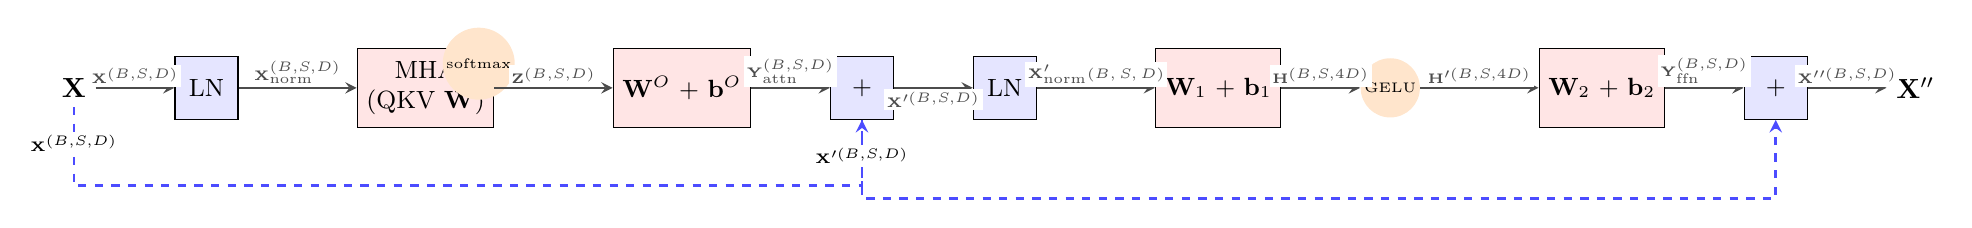
\begin{tikzpicture}[
    % 1. 스타일 정의
    >=stealth, 
    vertex/.style={draw, fill=blue!10, rectangle, minimum size=8mm, font=\small}, 
    opbox/.style={draw, fill=red!10, rectangle, minimum width=1.0cm, minimum height=1cm, font=\small, align=center}, % 압축된 너비
    nonlinear/.style={fill=orange!20, circle, inner sep=1pt, minimum size=5mm, font=\tiny}, 
    tensordim/.style={font=\tiny, fill=white, inner sep=1pt}, 
    res/.style={->, line width=1pt, blue!70, dashed}, 
    flow/.style={->, thick, black!70} 
]

    % =================================================================
    % I. Multi-Head Attention (MHA) 블록 정의 (간격 최소화 유지)
    % =================================================================
    \node (Input) at (0, 0) {$\mathbf{X}$};
    \node[vertex] (LN1) [right=1.0cm of Input] {LN}; 
    \node[opbox] (MHA) [right=1.5cm of LN1] {MHA\\(QKV $\mathbf{W}$)}; 
    \node[opbox] (WO) [right=1.5cm of MHA] {$\mathbf{W}^O$ + $\mathbf{b}^O$}; 
    \node[vertex] (Add1) [right=1.0cm of WO] {+}; 
    \node[nonlinear] (NL1) at ($(MHA.north east) + (-0.2, -0.2)$) {softmax}; 

    % =================================================================
    % II. Feed-Forward Network (FFN) 블록 정의 (간격 최소화 유지)
    % =================================================================
    \node[vertex] (LN2) [right=1.0cm of Add1] {LN}; 
    \node[opbox] (W1) [right=1.5cm of LN2] {$\mathbf{W}_1$ + $\mathbf{b}_1$}; 
    \node[nonlinear] (NL2) [right=1.0cm of W1] {GELU}; 
    \node[opbox] (W2) [right=1.5cm of NL2] {$\mathbf{W}_2$ + $\mathbf{b}_2$}; 
    \node[vertex] (Add2) [right=1.0cm of W2] {+}; 
    \node (Output) [right=1.0cm of Add2] {$\mathbf{X}''$};

    % =================================================================
    % 텐서 흐름 (Flow Lines) 및 차원 명시
    % =================================================================
    \draw[flow] (Input) -- (LN1) node[tensordim, midway, above] {$\mathbf{X}^{(B, S, D)}$};
    \draw[flow] (LN1) -- (MHA) node[tensordim, midway, above] {$\mathbf{X}_{\text{norm}}^{(B, S, D)}$};
    \draw[flow] (MHA) -- (WO) node[tensordim, midway, above] {$\mathbf{Z}^{(B, S, D)}$};
    \draw[flow] (WO) -- (Add1) node[tensordim, midway, above] {$\mathbf{Y}_{\text{attn}}^{(B, S, D)}$};
    \draw[flow] (Add1) -- (LN2) node[tensordim, midway, below] {$\mathbf{X}'^{(B, S, D)}$};
    \draw[flow] (LN2) -- (W1) node[tensordim, midway, above] {$\mathbf{X}'_{\text{norm}} (B, S, D)$}; 
    \draw[flow] (W1) -- (NL2) node[tensordim, midway, above] {$\mathbf{H}^{(B, S, 4D)}$};
    \draw[flow] (NL2) -- (W2) node[tensordim, midway, above] {$\mathbf{H}'^{(B, S, 4D)}$};
    \draw[flow] (W2) -- (Add2) node[tensordim, midway, above] {$\mathbf{Y}_{\text{ffn}}^{(B, S, D)}$};
    \draw[flow] (Add2) -- (Output) node[tensordim, midway, above] {$\mathbf{X}''^{(B, S, D)}$};

    % =================================================================
    % III. 잔차 연결 (Residual Connections) 명시
    % =================================================================
    \draw[res] (Input.south) -- ++(0, -1.0) -| (Add1.south);
    \node[tensordim, above] at ($(Input.south)+(0, -0.6)$) {$\mathbf{X}^{(B, S, D)}$}; 

    \draw[res] (Add1.south) -- ++(0, -1.0) -| (Add2.south);
    \node[tensordim, above] at ($(Add1.south)+(0, -0.6)$) {$\mathbf{X}'^{(B, S, D)}$}; 

\end{tikzpicture}
} % resizebox 명령어 닫음

\end{document}
